\documentclass[a4paper]{article}
\usepackage[a4paper, total={7in, 9in}]{geometry}
\usepackage{tikz}
\usepackage{booktabs}
\usepackage{float}
\setlength{\parindent}{0pt}
\begin{document}
\title{Project Management Plan Template Example}
\date{}
\maketitle
\textbf{Project Name:} Just-In-Time Training Project
\section{Introduction/Overview}

\begin{tikzpicture}
\draw (0,0) rectangle (18,2) node[pos=.5] {Introduce reader to project and provide background};
\end{tikzpicture}

\section{Project Organisation}
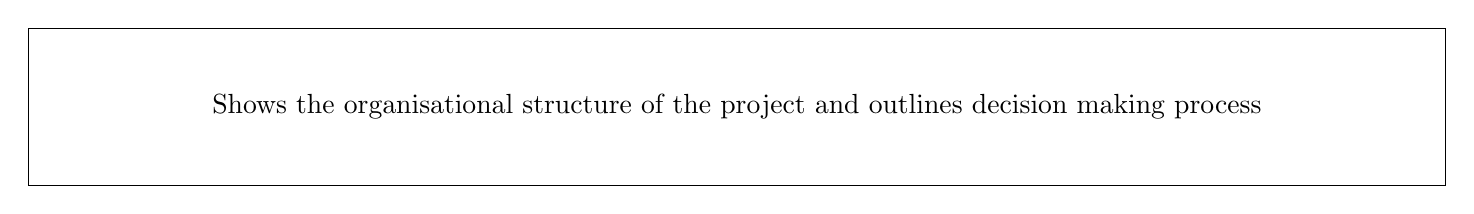
\begin{tikzpicture}
\draw (0,0) rectangle (18,2) node[pos=.5] {Shows the organisational structure of the project and outlines decision making process};
\end{tikzpicture}
\begin{figure}[h]
\centering
\includegraphics[scale=0.5]{proj_org}
\end{figure}

\section{Management}

\begin{tikzpicture}
\draw (0,0) rectangle (18,2) node[pos=.5] {Outlines requirements and processes for management review, and supplier choice};
\end{tikzpicture}

\section{Technical Processes}
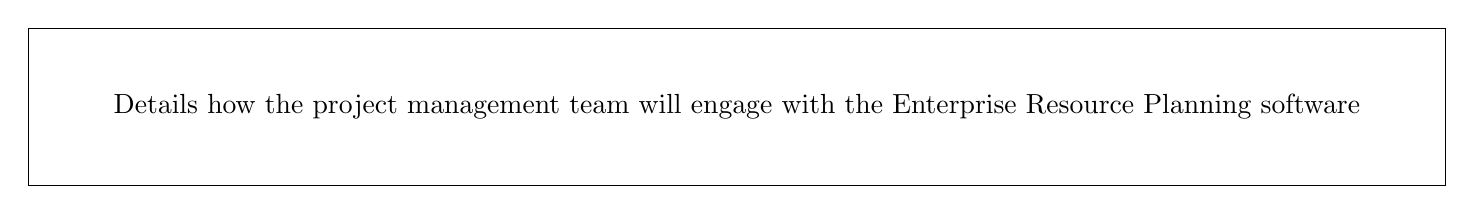
\begin{tikzpicture}
\draw (0,0) rectangle (18,2) node[pos=.5] {Details how the project management team will engage with the Enterprise Resource Planning software};
\end{tikzpicture}

\section{Work to be Performed}
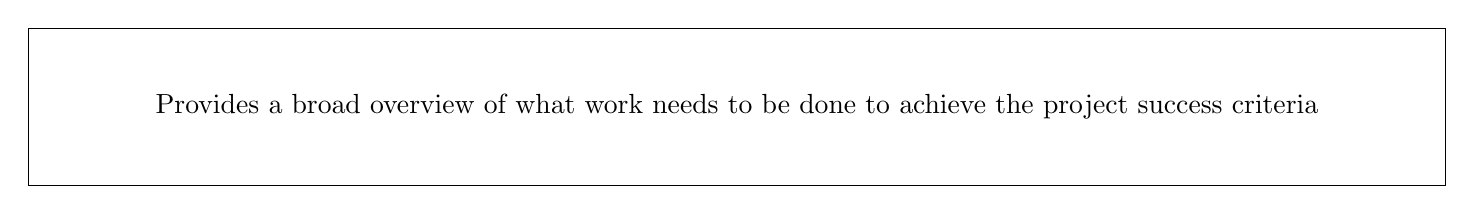
\begin{tikzpicture}
\draw (0,0) rectangle (18,2) node[pos=.5] {Provides a broad overview of what work needs to be done to achieve the project success criteria};
\end{tikzpicture}

\section{Schedule Information}

\begin{tikzpicture}
\draw (0,0) rectangle (18,2) node[pos=.5] {Provides an overview of the project schedule to completion};
\end{tikzpicture}

\section{Budget Information}

\begin{tikzpicture}
\draw (0,0) rectangle (18,2) node[pos=.5] {Provides information on the costs associated with the project};
\end{tikzpicture}

\section{Reference to Other Project Planning Documents}

\begin{tikzpicture}
\draw (0,0) rectangle (18,2) node[pos=.5] {Provides reference to any supporting documentation};
\end{tikzpicture}
\end{document}